\documentclass{article}
\usepackage{tikz}
\usetikzlibrary{arrows.meta}

\begin{document}

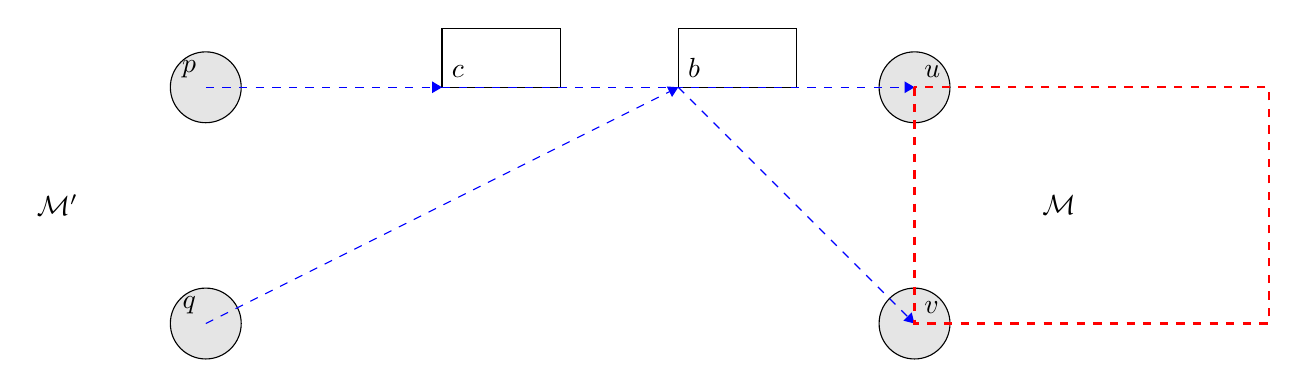
\begin{tikzpicture}[scale=1.5]
    % Define coordinates
    \coordinate (p) at (0, 0);
    \coordinate (q) at (0, -2);
    \coordinate (c) at (2, 0);
    \coordinate (b) at (4, 0);
    \coordinate (u) at (6, 0);
    \coordinate (v) at (6, -2);

    % Draw circles
    \draw[fill=black!10] (p) circle (0.3);
    \draw[fill=black!10] (q) circle (0.3);
    \draw[fill=black!10] (u) circle (0.3);
    \draw[fill=black!10] (v) circle (0.3);

    % Draw rectangles
    \draw[fill=white] (c) rectangle ++(1, 0.5);
    \draw[fill=white] (b) rectangle ++(1, 0.5);

    % Draw dashed lines with arrows
    \draw[blue, dashed, -Triangle] (p) -- (c);
    \draw[blue, dashed, -Triangle] (q) -- (b);
    \draw[blue, dashed, -Triangle] (c) -- (u);
    \draw[blue, dashed, -Triangle] (b) -- (v);

    % Draw the red rectangle
    \draw[red, thick, dashed] (6, 0) rectangle ++(3, -2);

    % Draw the labels
    \node at (p) [above left] {$p$};
    \node at (q) [above left] {$q$};
    \node at (c) [above right] {$c$};
    \node at (b) [above right] {$b$};
    \node at (u) [above right] {$u$};
    \node at (v) [above right] {$v$};

    % Draw the labels M' and M
    \node at (-1, -1) [left] {$\mathcal{M}'$};
    \node at (7, -1) [right] {$\mathcal{M}$};
\end{tikzpicture}

\end{document}